\documentclass{article}
\usepackage{../fasy-hw}
\usepackage{algopseudocode}
\usepackage{graphics}

%% UPDATE these variables:
\renewcommand{\hwnum}{5}
\title{Advanced Algorithms, Homework \hwnum}
\author{Sarah Montalbano}
\collab{\todo{list your collaborators here}}
\date{due: Monday, 8 November 2021}

\begin{document}

\maketitle

This homework assignment should be
submitted as a single PDF file both to D2L and to Gradescope.

General homework expectations:
\begin{itemize}
    \item Homework should be typeset using LaTex.
    \item Answers should be in complete sentences and proofread.
    \item You will not plagiarize, nor will you share your written solutions
        with classmates.
    \item List collaborators at the start of each question using the
        \texttt{collab} command.
    \item Put your answers where the \texttt{todo} command currently is (and
        remove the \texttt{todo}, but not the word \texttt{Answer}).
    \item If you are asked to come up with an algorithm, you are
        expected to give an algorithm that beats the brute force (and, if possible, of
        optimal time complexity). With your algorithm, please provide the following:
        \begin{itemize}
            \item \emph{What}: A prose explanation of the problem and the algorithm,
                including a description of the input/output.
            \item \emph{How}: Describe how the algorithm works, including giving
                psuedocode for it.  Be sure to reference the pseudocode
                from within the prose explanation.
            \item \emph{How Fast}: Runtime, along with justification.  (Or, in the
                extreme, a proof of termination).
            \item \emph{Why}: Statement of the loop invariant for each loop, or
                recursion invariant for each recursive function.
        \end{itemize}
\end{itemize}

\collab{\todo{}}
\nextprob{The Skyline Problem}

You are in Camden, NJ waiting for the ferry across the river to
get into Philadelphia, and are looking at the skyline.  You take a photo, and notice that each building
has the silhouette of a rectangle.  Suppose you  represent each building $b$ as a
triple $(x_b^{(1)},x_b^{(2)},y_b)$, where the building can be seen from $x_b^{(1)}$ to $x_b^{(2)}$
horizontally and has a height of $y_b$.  Let $\mathtt{rect(b)}$ be the set of
points inside this rectangle (including the boundary).  Let $\mathtt{buildings}$
be a set of $n$ such triples representing buildings. Design an algorithm that takes $\mathtt{buildings}$ as input, and
returns the skyline, where the skyline is a sequence of~$(x,y)$ coordinates
defining $\cup_{b \in \mathtt{buildings}} \mathtt{rect}(b)$.  The output should
start with $(\min_b{x_b^{(1)}},0)$ and end with $(\max_b{x_b^{(1)}},0)$.

\paragraph{Answer}
\todo{}

\collab{\todo{}}
\nextprob{Longest Increasing Subsequence}

Next, we consider the problem of finding the longest increasing subsequence.

\begin{enumerate}
    \item
        Walk through one of the exponential time algorithms to compute the
        Longest Increasing Subsequence (LIS) for the input: $\left[ 1, 7, 6, 11,
        3, 11 \right]$.  You can use either the algorithm presented in 2.6 or
        the algorithm presented in 2.7.

        \paragraph{Answer} \todo{}

    \item
        Walk through the algorithm (on the same input) using the Dynamic Programming algorithm
        present in Section 3.6.

        \paragraph{Answer} \todo{}

\end{enumerate}

\collab{\todo{}}
\nextprob{Decrementing Function}

Consider the algorithm \textsc{StrongComponents} given on in Figure 6.15 of the
textbook. Notationally, use $G=(V,E)$ for the graph and let $n=|V|$ and $m=|E|$.
In the for loop, there are at most $n$ vertices that will be
considered. So, that loop will terminate in $O(m)$ iterations.
Use a decrementing function to prove that the while loop terminates.

\paragraph{Answer}
\todo{}

\collab{\todo{}}
\nextprob{Kruskal}

Walk through Kruskal's algorithm, using the graph in Figure 7.7 (left) of the
textbook.  Label the center vertex $a$, the other red vertex $b$, and the
remainder $c$ through $g$ in counter-clockwise order.  You should use the
union-find data structure, with both ``heuristics.''

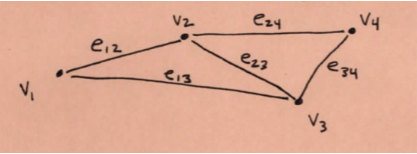
\includegraphics[scale=.10]{graph.jpg}

\begin{algorithmic}
\Function{KruskalWalkthrough}{V, E}
\State Sort E by increasing weight
\State E = [2, 3, 4, 5, 8, 10, 12, 14, 16, 18, 26, 30]
\EndFunction
\end{algorithmic}

\paragraph{Answer}
\todo{}

\collab{\todo{}}
\nextprob{Maximum and Minimum Edges in Cycles}

Chapter 7, Question 1

\begin{enumerate}[(a)]

    \item Excluding Maximum Weight Edges.

        \paragraph{Answer}
        \todo{}


    \item Including Minimum Weight Edges.

        \paragraph{Answer}
        \todo{}

\end{enumerate}


\collab{\todo{}}
\nextprob{Maximum Weight Spanning Tree}

Chapter 7, Question 4, Part(a).

\paragraph{Answer}
\todo{}



\end{document}
